\section{Appendix}
\label{sec:appendix}

\subsection{ADQL Query for the SIMBAD Database}
\label{sec:simbad-query}

% Full resolution input image

% Matched stars labeled on image

\begin{lstlisting}[language=SQL, caption={
  ADQL query for the SIMBAD database to find stars in the field of view of the input image.
  "Star.." stands for "star or any sub category of star". The query can be executed at
  \url{https://simbad.cds.unistra.fr/simbad/sim-tap/}.
}, label={lst:simbad-query}]
SELECT COUNT(*)
FROM basic JOIN flux ON oidref = oid
WHERE otype = 'Star..'
      AND filter = 'V'
      AND flux < 8.0
      AND CONTAINS(POINT('ICRS', RA, DEC), BOX('ICRS', 312.708, 60.171, 64, 45)) = 1;
\end{lstlisting}

\newpage

\subsection{Histograms of Predicted Magnitudes}

\begin{figure}[htbp]
  \centering
  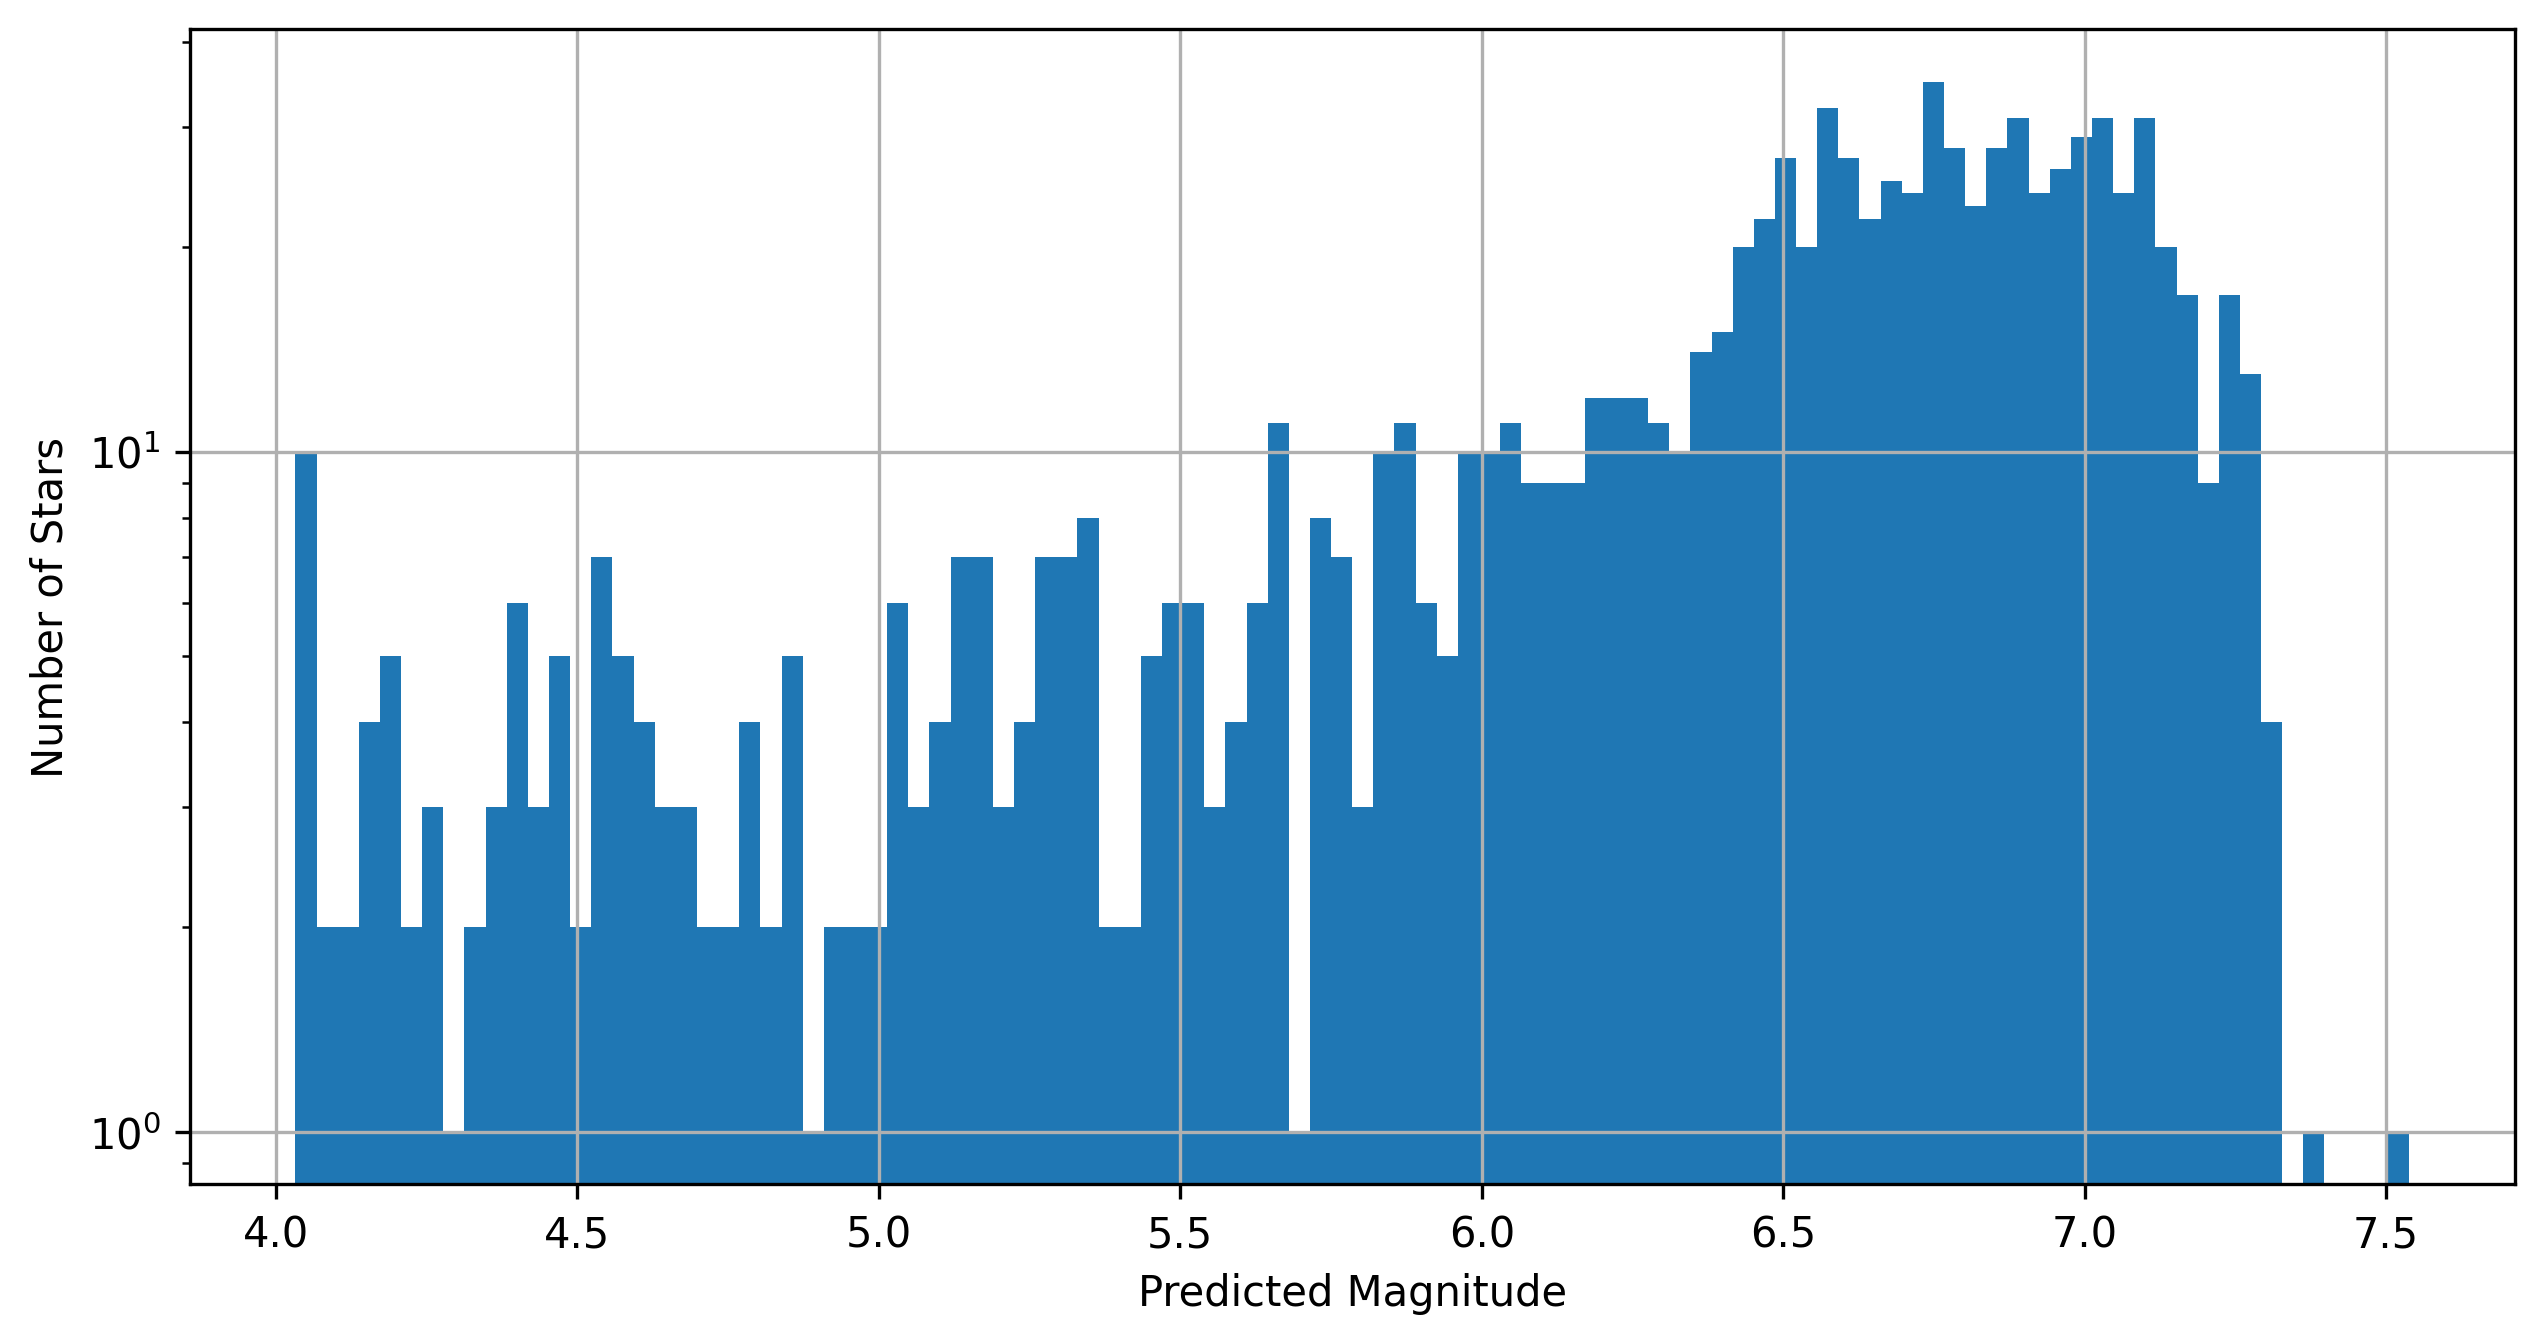
\includegraphics[width=.8\linewidth]{histogram_predicted_magnitudes.png}
  \caption{Histogram of the predicted magnitudes of stars in the input image.}
  \label{fig:hist-predicted-magnitudes}
\end{figure}

\begin{figure}[htbp]
  \centering
  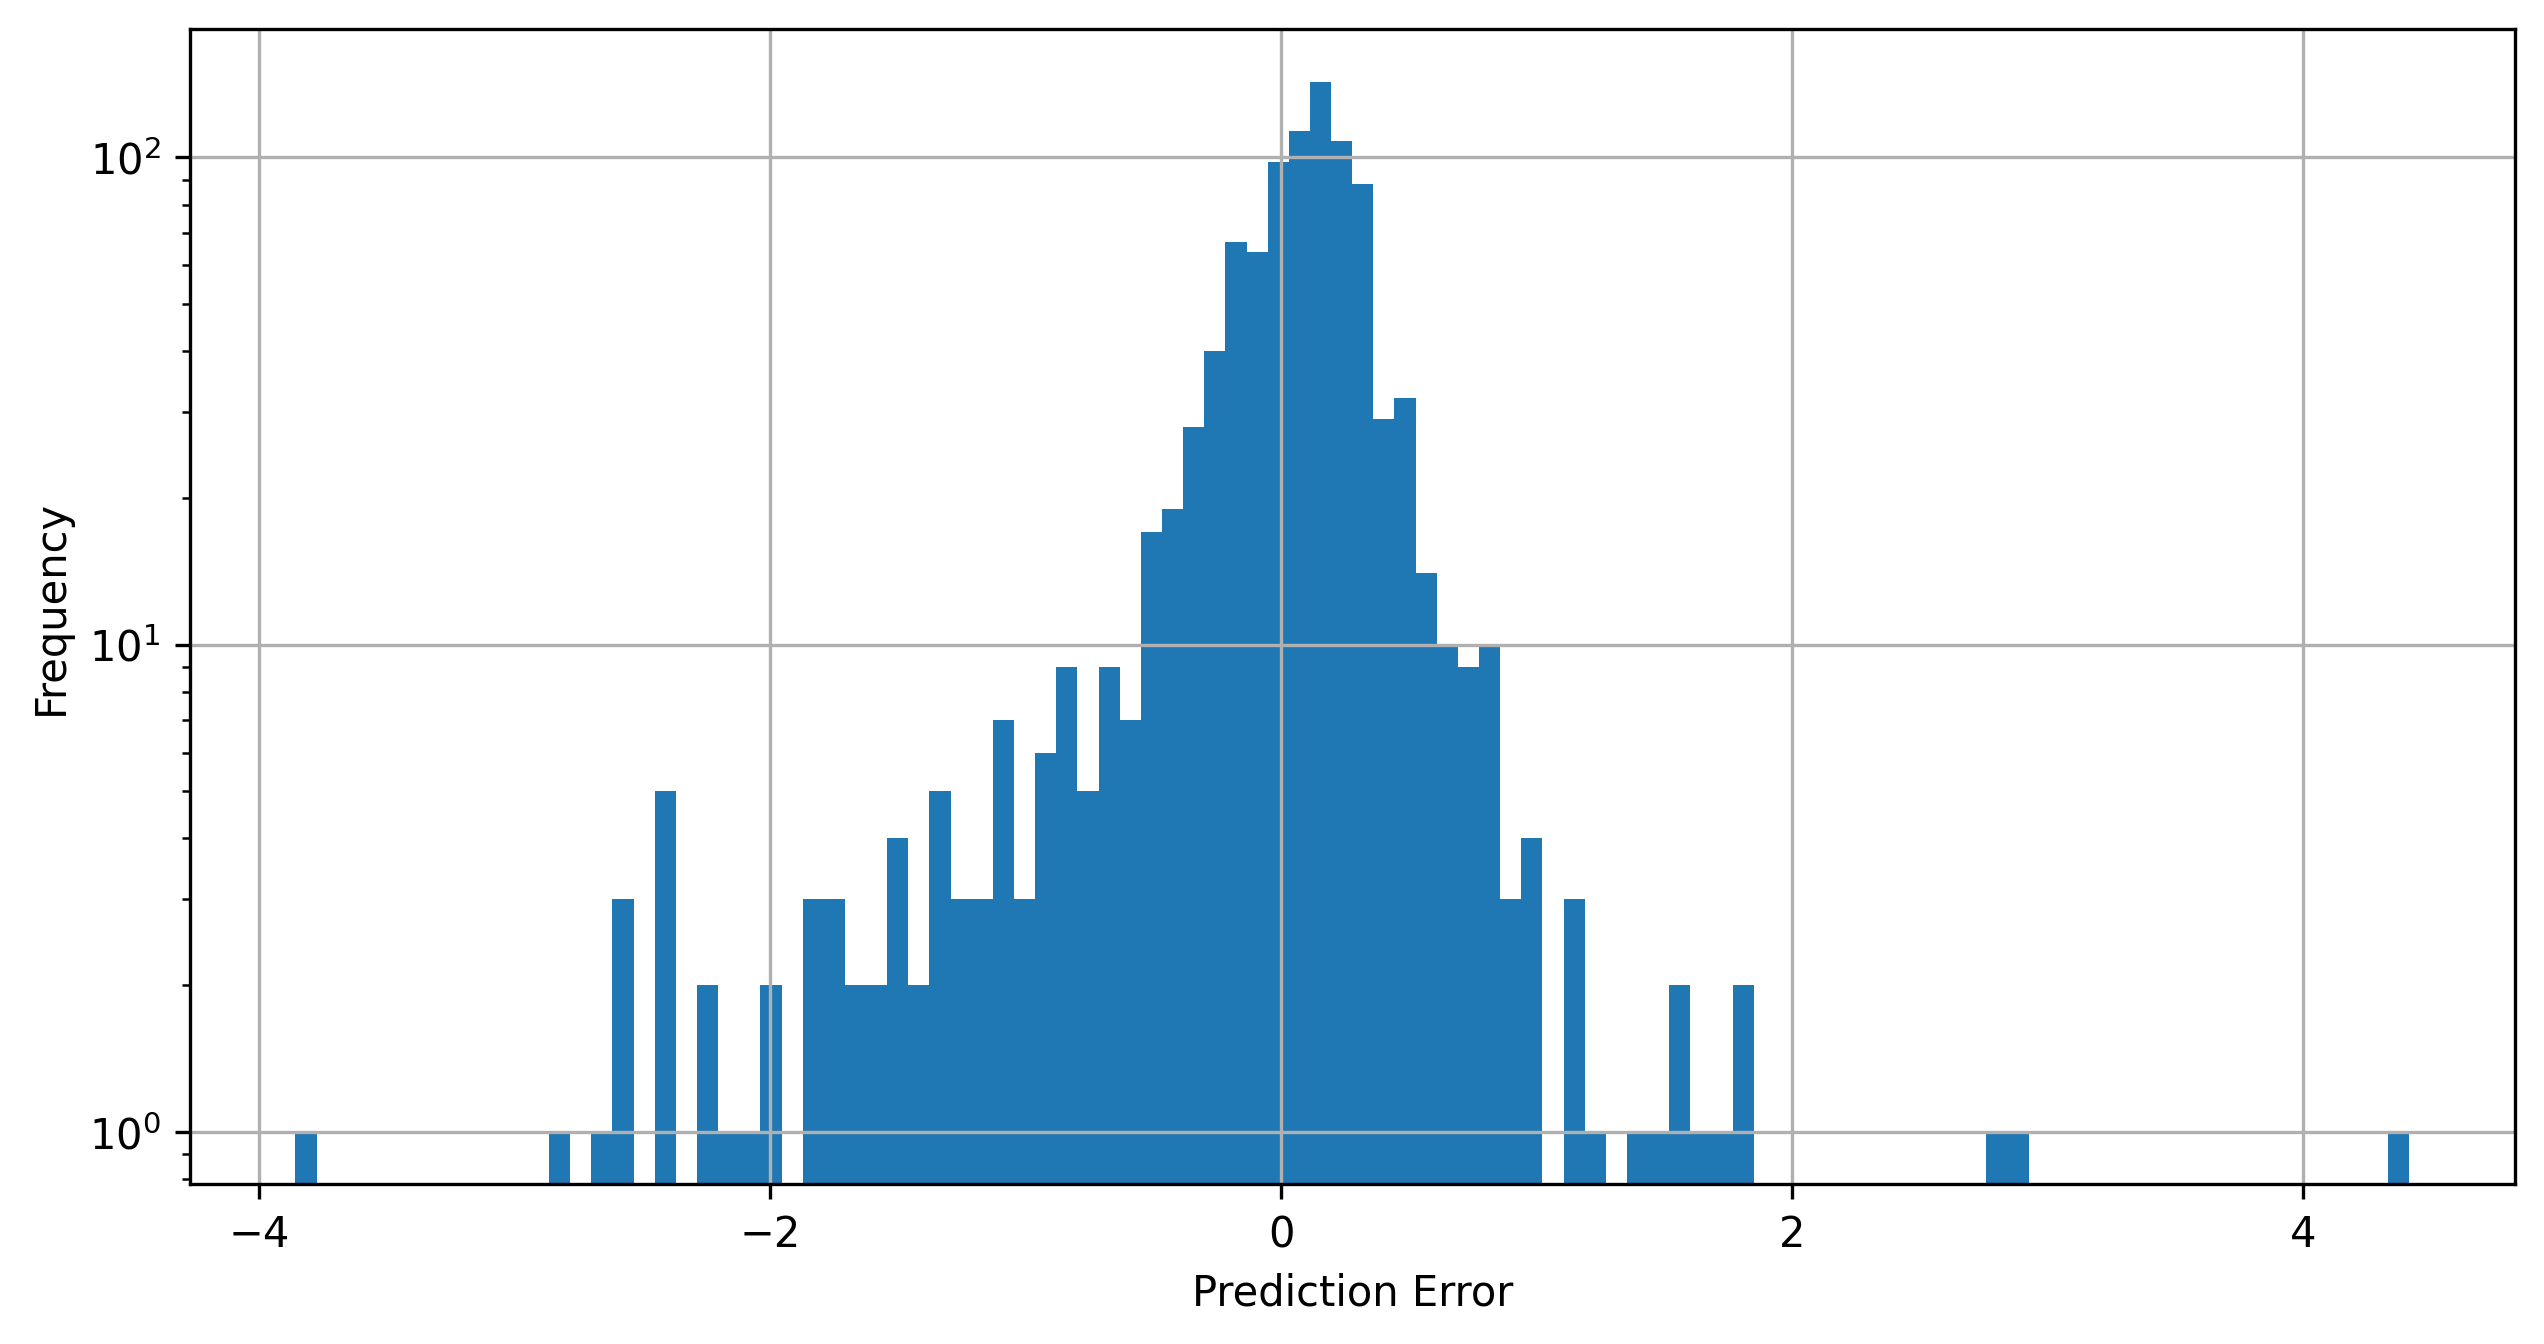
\includegraphics[width=.8\linewidth]{histogram_prediction_error.png}
  \caption{Histogram of the prediction error of the magnitudes of stars in the input image.}
  \label{fig:hist-predicted-error}
\end{figure}

\newpage

\subsection{Output of the Astrometry.net Service}

\begin{figure}[htbp]
  \centering
  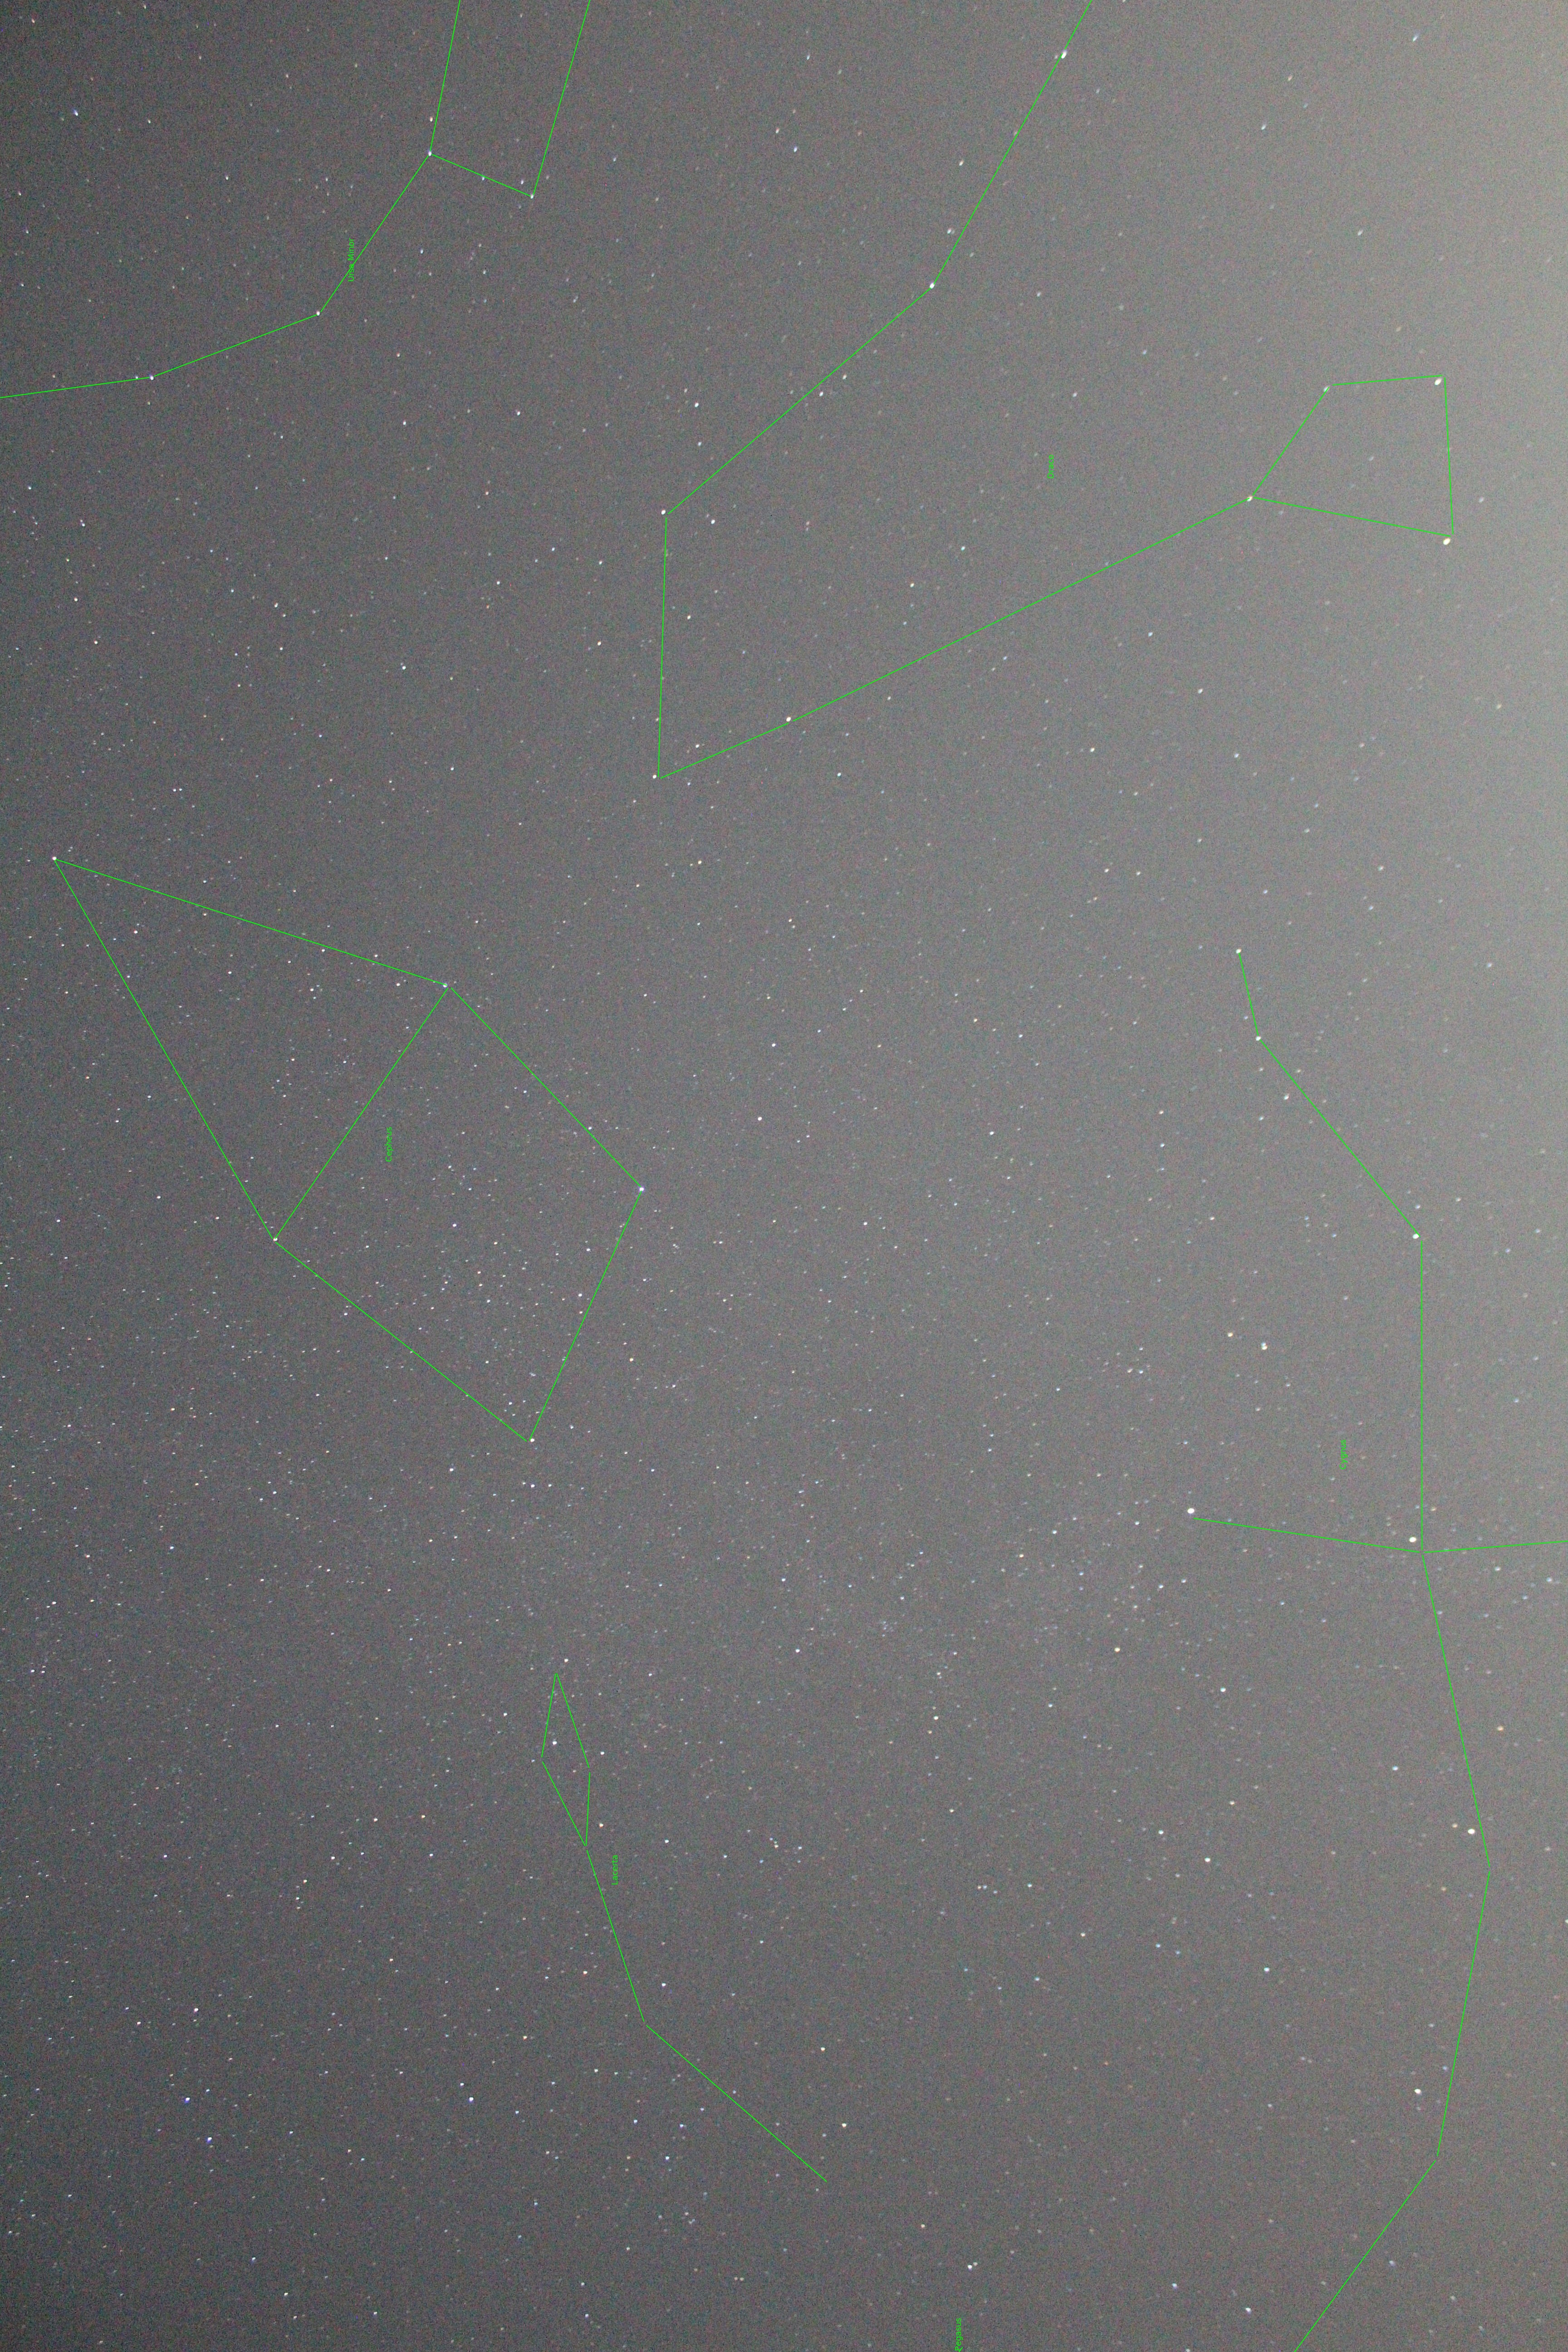
\includegraphics[width=.6\linewidth]{annotated.jpeg}
  \caption{Output of the Astrometry.net service for the input image. Find the results\\
    online at \url{https://nova.astrometry.net/user\_images/11597239\#annotated}.}
  \label{fig:astrometry-output}
\end{figure}